% Created 2021-09-01 Wed 16:36
% Intended LaTeX compiler: pdflatex
\documentclass[11pt]{article}
\usepackage[utf8]{inputenc}
\usepackage[T1]{fontenc}
\usepackage{graphicx}
\usepackage{grffile}
\usepackage{longtable}
\usepackage{wrapfig}
\usepackage{rotating}
\usepackage[normalem]{ulem}
\usepackage{amsmath}
\usepackage{textcomp}
\usepackage{amssymb}
\usepackage{capt-of}
\usepackage{hyperref}
\author{JT Laune}
\date{\today}
\title{Research Notes/TODOs}
\hypersetup{
 pdfauthor={JT Laune},
 pdftitle={Research Notes/TODOs},
 pdfkeywords={},
 pdfsubject={},
 pdfcreator={Emacs 27.2 (Org mode 9.4.6)}, 
 pdflang={English}}
\begin{document}

\maketitle
\tableofcontents

-\textbf{- mode:org -}-
\section{capture}
\label{sec:org67e5718}
\subsection{{\bfseries\sffamily TODO} run longer integration for \(Te1/Te2=0.1\)}
\label{sec:orga8e608c}
\subsection{{\bfseries\sffamily TODO} write why Dpomeg to 0}
\label{sec:org6c8875b}
\subsection{{\bfseries\sffamily TODO} comment about setting \(Tw0=10\) kyr}
\label{sec:orgd10b7d2}
\subsection{{\bfseries\sffamily TODO} comment on loose terminology}
\label{sec:org4b70122}
\subsection{DONES}
\label{sec:org180a494}
\subsubsection{{\bfseries\sffamily DONE} Solve for Tej (ej?) if Tek = infty algebraic/numerical}
\label{sec:org52615aa}
\subsubsection{{\bfseries\sffamily DONE} Test different tolerance settings \& integrators for ecc decay}
\label{sec:org8fb3be1}
\begin{itemize}
\item plot avg(sin(theta)) for diff tol/integrators to see if numerical issue
\end{itemize}
\subsubsection{{\bfseries\sffamily DONE} Integrate a reasonable time for orbit evolution of q=0.001 for ecc decay}
\label{sec:org3f5a3ad}
\subsubsection{{\bfseries\sffamily DONE} solve analytical eq for e1/2d driving eccs}
\label{sec:org55cfc2b}
\subsubsection{{\bfseries\sffamily DONE} Test different Te1/Te2 ratios for ecc decay}
\label{sec:orgcb28c25}
\subsubsection{{\bfseries\sffamily DONE} read petigura 2019}
\label{sec:org7a59980}
\subsubsection{{\bfseries\sffamily DONE} read ragusa 2018}
\label{sec:orgc191839}
\section{Meetings}
\label{sec:org1497a99}
\subsection{\textit{[2021-08-27 Fri] } MEETING}
\label{sec:org1285e40}
\begin{enumerate}
\item fix equation 4
\item discuss plus/minus migrations, define 1/Tm = diff
\item fig 4 why not symmetric? put q inside fix y labels
\item fix figure 5 theta hat
\end{enumerate}
\subsection{\textit{[2021-08-20 Fri] } MEETING}
\label{sec:orgc888c31}
\begin{enumerate}
\item label all equations
\item Hhat to end
\item Include system parameters in captions
\item Fig 2 at beginning of 2.2
\begin{itemize}
\item example/answer -> then explain
\end{itemize}
\item check error bars if so then show example of large e variations
\item add analytic estimate to figure 5
\item erase w/o secular line in Figure 5
\item Figure 6 plot Delta pomega -180 to 180, not absolute value
\item Fewer dots/integrations for figures 4 and 5
\end{enumerate}
\subsection{\textit{[2021-08-12 Thu] } MEETING}
\label{sec:orgada5743}

\subsection{\textit{[2021-08-06 Fri] } MEETING}
\label{sec:org501b17f}
\begin{enumerate}
\item Mention K2-19 in intro/sec2
\item Integrate sec4 into sec3; it's not useful to fit the system exactly
\item seems like we reach a different equilibrium depending on initial
conditions
\item ecc driving ansatz -> robust alignment
\item possibly high initial eccentricities ? less robust? another channel?
\item Make analytical argument with the first 2 equilibrium equations
for the plot:
\begin{itemize}
\item |\(\Delta\varpi\)
\begin{center}
\begin{tabular}{}
\\
\uline{\uline{\uline{\uline{\uline{\uline{\uline{\_\_}}}}}}}\\
\end{tabular}
\end{center}
0.2  1  5 Te1/Te2
\end{itemize}
\end{enumerate}
\subsection{\textit{[2021-07-30 Fri] } MEETING}
\label{sec:orge37a360}
\begin{enumerate}
\item First do natural Te e/Te e->0
\item Section 2 standard picture
\item 1st thing show secular coupling, 1 example
\item section 2 like a recap, review, show why \(\Delta\varpi\to\pi\), with
small correction as a function of (q, Tw0)
\item make a detailed outline
\item section 3 consider toy model e1d>0, same parameters
\end{enumerate}
\subsubsection{Dong's outline sketch}
\label{sec:orgf5cc6e9}
\begin{enumerate}
\item Introduction
\item Recap of "standard" picture
\begin{itemize}
\item forces: e1/Te1, e2/Te2
\item cases
q=2
q=1
q=1/2
\item |e1eq, e2eq
\begin{center}
\begin{tabular}{}
\\
\uline{\uline{\uline{\uline{\uline{\uline{\uline{\_\_}}}}}}}\\
\end{tabular}
\end{center}
0.2  1  5 Te1/Te2
\item |\(\Delta\varpi\)
\begin{center}
\begin{tabular}{}
\\
\uline{\uline{\uline{\uline{\uline{\uline{\uline{\_\_}}}}}}}\\
\end{tabular}
\end{center}
0.2  1  5 Te1/Te2
\end{itemize}
\item Toy Model, e1d>0
\begin{itemize}
\item forces: (e1-e1d)/Te1, e2/Te2
\item cases
q=2
q=1
q=1/2
\item |e1eq, e2eq
\begin{center}
\begin{tabular}{}
\\
\uline{\uline{\uline{\uline{\uline{\uline{\uline{\_\_}}}}}}}\\
\end{tabular}
\end{center}
0.2  1  5 Te1/Te2
\item |\(\Delta\varpi\)
\begin{center}
\begin{tabular}{}
\\
\uline{\uline{\uline{\uline{\uline{\uline{\uline{\_\_}}}}}}}\\
\end{tabular}
\end{center}
0.2  1  5 Te1/Te2
\end{itemize}
\item "Fancy" Hamiltonian
\end{enumerate}
\subsection{\textit{[2021-07-23 Fri] } MEETING}
\label{sec:org24028dc}
\begin{enumerate}
\item try q \textasciitilde{} 1 for T >> Te2 to see if equilibrium is reached
\item try runs with the "story" of the capture process:
\begin{itemize}
\item for alignment must have e\textsubscript{20} > mu\textsubscript{1}\textsuperscript{2}/3 and e\textsubscript{10} > mu\textsubscript{2}\textsuperscript{2}/3 to
avoid capture into theta1/2 resonances
\item must have hat(e) within resonance capture range for hat(theta)
\item damping stops before theta1/2 equilibrium is reached
\end{itemize}
\end{enumerate}
\subsubsection{Plans for draft of paper}
\label{sec:orgc8ec857}
\begin{enumerate}
\item Introduction
\begin{itemize}
\item K2-19 is puzzling in light of anti-alignment outcome
\end{itemize}
\item Summarize q first
\begin{itemize}
\item example, stable case T to infty
\item secular term modification "canonical case"
\item why anti-alignment, small secular effects
\end{itemize}
\item TP case (possibly sec1 or in appendix if not relevant)
\end{enumerate}
\subsubsection{Plans for research talk}
\label{sec:org230fbe8}
\begin{itemize}
\item K2-19 system
\item Subresonances
\item reproducing TP results with q=1000
\begin{itemize}
\item analytic equilibrium results, not a true equilibrium
\end{itemize}
\item Driving eccentricities for q\textasciitilde{}O(1) cases
\begin{itemize}
\item reproducing K2-19 alignment
\item disucssion of Tei physics?
\end{itemize}
\end{itemize}
\subsection{\textit{[2021-07-16 Fri] } MEETING}
\label{sec:orgc3bd322}
\begin{enumerate}
\item Solve for Tej if Tek = infty algebraic/numerical
\item Only drive the larger planet's eccentricity to be nonzero
\item Look at observations of \(\Delta\varpi\). How do they measure it?
\begin{enumerate}
\item are there any observed aligned cases in the literature?
\item If so, this is counter to the strong conclusion that the
resonance is resilient to the the Te1/Te2 ratio and that in
resonance the planets are always anti-aligned. \textbf{This could be the
argument for your paper.}
\end{enumerate}
\item Try comparable mass for e2d->0.1, maybe q=2
\item Ragusa 2018 eccentricity evolution during planet disk interaction
\begin{enumerate}
\item Long hydro simulation
\end{enumerate}
\item \textbf{Problem of why q=1000 affects teh larger planet so much!!!!}
\begin{enumerate}
\item \textbf{Integrate a reasonable time for orbit evolution of q=0.001}
\item Compare Te1/Te2 reasonable case to crazy large case
\item Compare Te2 timescale to theta2 resonance timescale. Is it
constant on a reasonable timescale of integration?
\item Run for only a few Te of the smaller planet
\item Try BS integrator \& vary tolerance while plotting
avg(sin(theta)) to see if results agree and it's not the code's
fault
\end{enumerate}
\end{enumerate}
\subsection{\textit{[2021-07-09 Fri] } MEETING}
\label{sec:orgc1afabe}
\begin{enumerate}
\item It seems like the secular terms don't matter that much for the
q\textasciitilde{}[0.1-1] case for comparable masses
\item For more extreme mass ratios, such as q\textasciitilde{}[0.001-0.01], dynamics may
be more interesting
\begin{itemize}
\item in this regime Te2 is an arbitrary \emph{parameter} because a massive
planet's eccentricity damping will not be identical to a very
small neighbor
\item Gap opening planet, sustained eccentricity, negative Te2?
\end{itemize}
\item If we are writing a paper, what comes next?
\begin{itemize}
\item brief introduction of TP case
\item Parameter study of q\textasciitilde{}[0,1e-2], Te2 parameter, how this relates to
apsidal alignment/equilibrium eccentricity
\end{itemize}
\item Papers mentioned:
\begin{itemize}
\item Chelsea Huang Warm Jupiter Neighbors, Wasp-47 system
\end{itemize}
\item \textbf{Big picture}:
\begin{itemize}
\item What happens to a smaller (<\textasciitilde{}1\%) mass planet when approaching a MMR with a massive planet?
\item How does this relate to apsidal alignment?
\end{itemize}
\end{enumerate}
\subsubsection{Laetitia's equilibrium plots:}
\label{sec:orgea52c29}
\begin{center}
\includegraphics[width=.9\linewidth]{ltximg/Alignment.png}
\end{center}
\begin{center}
\includegraphics[width=.9\linewidth]{ltximg/Alignment_weakerdamping.png}
\end{center}
\subsubsection{{\bfseries\sffamily DONE} Read Huang paper}
\label{sec:org1cc6f77}
\subsubsection{{\bfseries\sffamily DONE} Get equilibrium solving code working you idiot}
\label{sec:orgad27dc0}
\begin{itemize}
\item look at extreme mass ratios
\item how do secular terms change the behavior?
\end{itemize}
\subsubsection{{\bfseries\sffamily DONE} Find a good parameter range for q, Te2, etc}
\label{sec:org57626be}
\subsubsection{{\bfseries\sffamily DONE} test parameter space with time-dependent numerical runs}
\label{sec:org9e258ef}
\begin{itemize}
\item in effort to answer \#5 above
\end{itemize}
\subsection{\textit{[2021-07-02 Fri] } MEETING}
\label{sec:orgc601e0d}
\emph{I think I am stupid}
\begin{enumerate}
\item Redo xu 2018 equations 16-18 but with the secular terms to see
where equilibrium is, make the same plots
\item Compare numerical results of equilibrium with secular terms turned
off to see the difference
\end{enumerate}
\section{Equations pdfs}
\label{sec:orgb1c3661}
\begin{center}
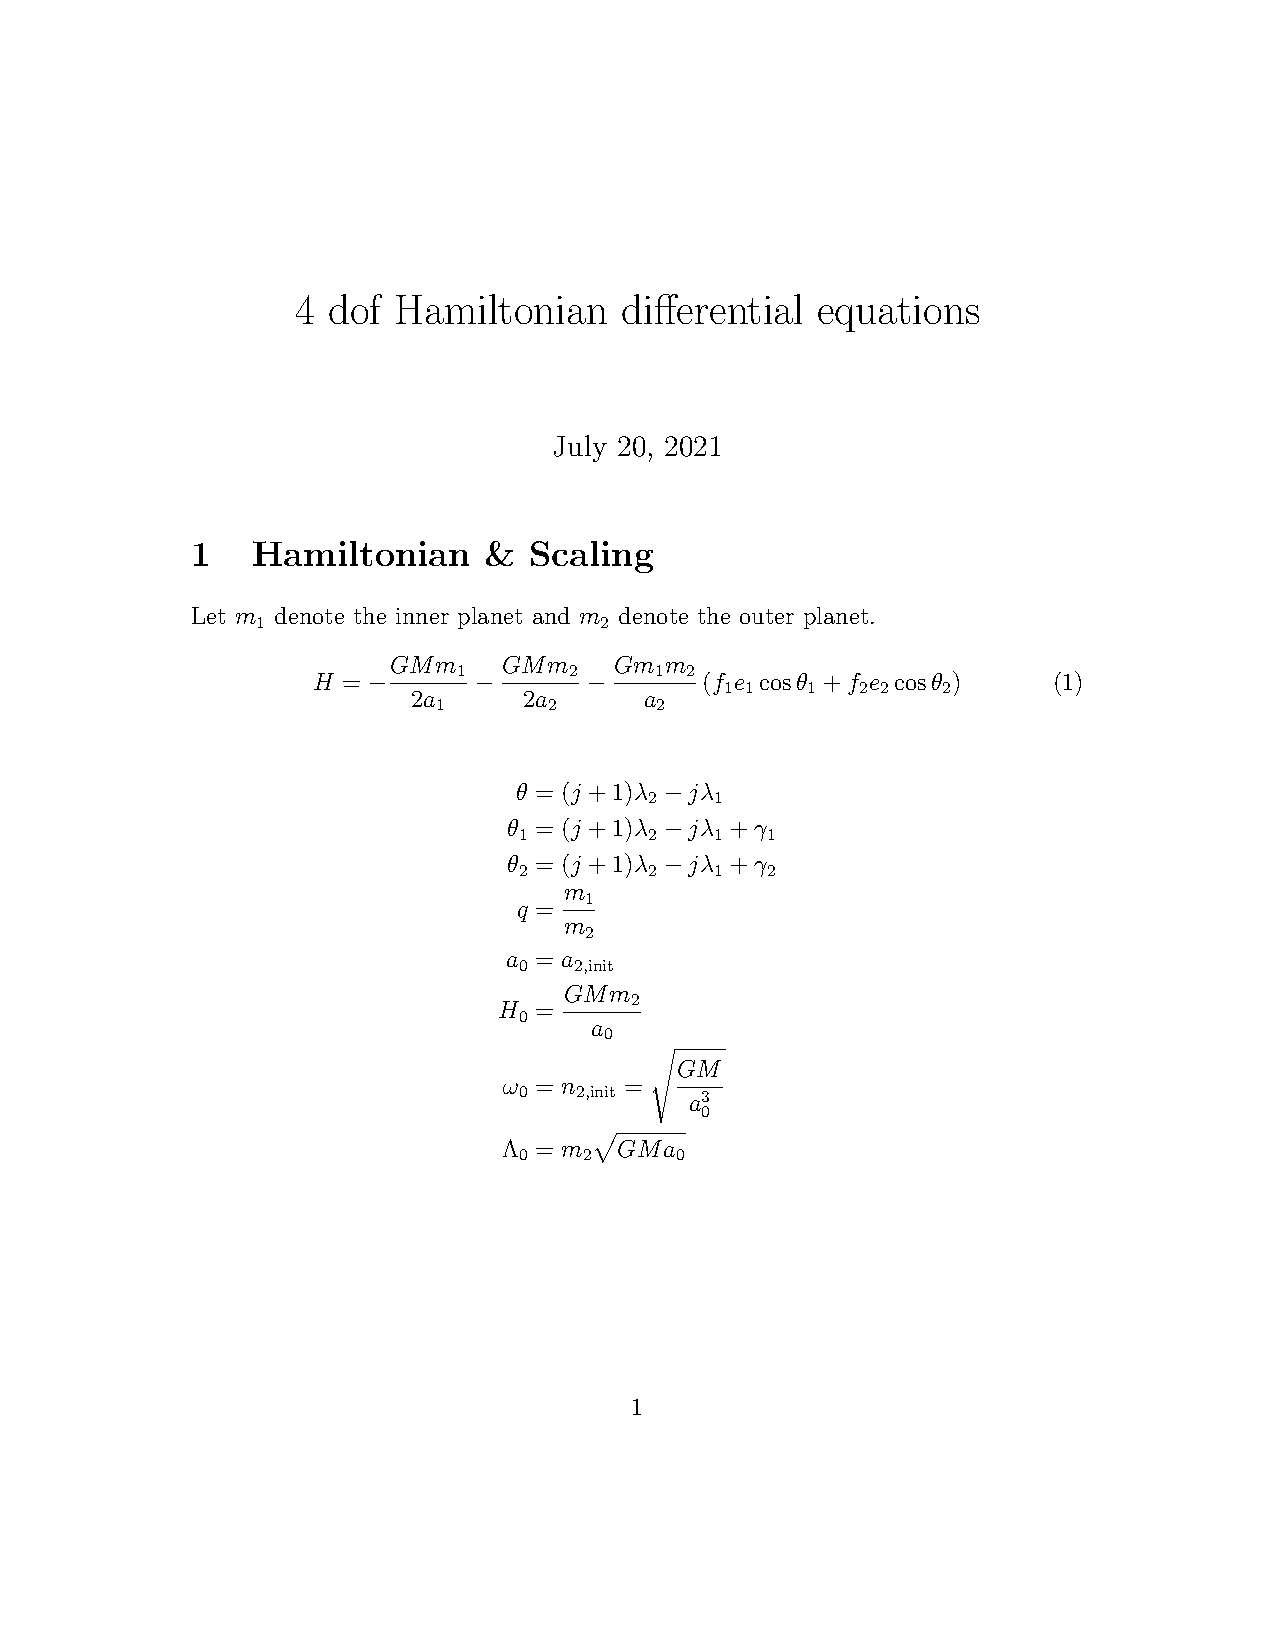
\includegraphics[width=.9\linewidth]{/home/jtlaune/multi-planet-architecture/docs/4dof-pdf/4dof_diffeqs.pdf}
\end{center}
\subsection{coefficients}
\label{sec:org2adb792}
\begin{verbatim}
sys.path.append("/home/jtlaune/multi-planet-architecture/")
from helper import *
alpha_0 = (j/(j+1))**(2./3.)
f1 = -A(alpha_0, j)
f2 = -B(alpha_0, j)
f3 = C(alpha_0)
f4 = D(alpha_0)
print([f"{fi:0.2f}" for fi in [f1, f2, f3, f4]])
\end{verbatim}

\section{Relevant Observed systems\hfill{}\textsc{ATTACH}}
\label{sec:orge5634db}
\subsection{K2-19 b \& c; Petigura et al. (2019)}
\label{sec:org64ea1f1}
\begin{itemize}
\item M\textsubscript{star} = 0.88 Msun
\item Pb = 7.9222d Pc = 11.8993d
\item Mb = 32.4ME Mc = 10.8ME
\item mu1 = 1.11e-4 mu2 = 3.69e-5 q = 3.00
\item e\textsubscript{b} = 0.20 e\textsubscript{c} = 0.21
\item x\textsubscript{b} = sqrt(e\textsubscript{b})*cos(varpi\textsubscript{b}) = 0.02
x\textsubscript{b} = sqrt(e\textsubscript{b})*sin(varpi\textsubscript{b}) = -0.44
\item x\textsubscript{c} = sqrt(e\textsubscript{c})*cos(varpi\textsubscript{c}) = 0.04
x\textsubscript{c} = sqrt(e\textsubscript{c})*sin(varpi\textsubscript{c}) = -0.46
\item Dvarpi\textsubscript{bc} = 2+-2 deg \textasciitilde{} 0.
\end{itemize}
\subsection{Huang et al. (2016)}
\label{sec:org92cd25b}
\begin{center}
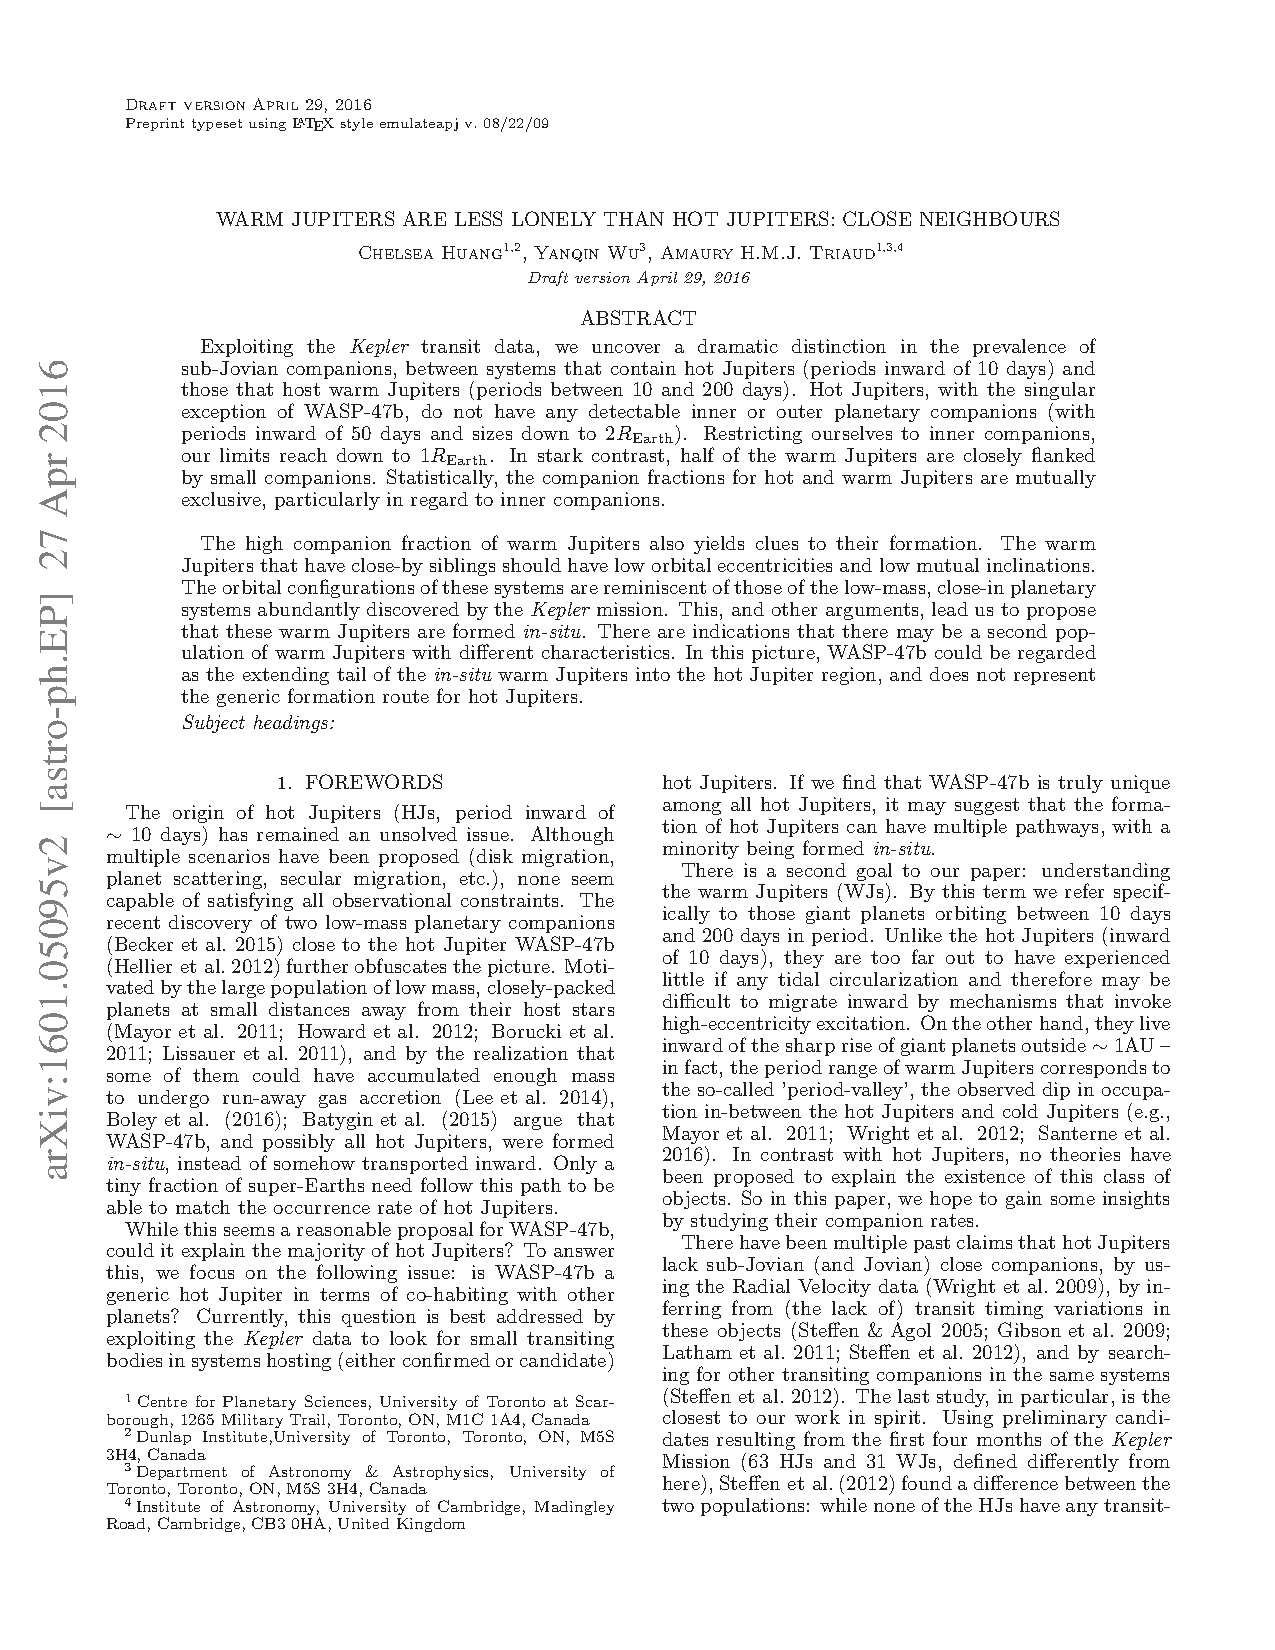
\includegraphics[width=.9\linewidth]{papers/huang-2016-WJneighbors.pdf}
\end{center}
:ID:       9ac2be99-7caa-47bf-b897-7babb34634a7
\begin{center}
\includegraphics[width=.9\linewidth]{/home/jtlaune/multi-planet-architecture/notes/2021-07-14_14-34-29_screenshot.png}
\end{center}
\subsubsection{Kepler-30 q\textasciitilde{}0.019, q\textasciitilde{}26}
\label{sec:org8a50bc3}
Panichi et al. (2017)
\url{https://arxiv.org/pdf/1707.04962.pdf}
b,c near 2:1 first order, q\textasciitilde{}0.019
all transiting
\emph{from exoplanet catalog:}
b 11.3 Me 0.18au 29.3 days e=0.04
c 2.01 Mj 0.3au 60.3 days e=0.01
d 23.1 Me 0.5au 143.3 days e=0.02
\subsubsection{Wasp-47}
\label{sec:orga4b09f8}
b 1.1 Mj
c 1.6 Mj
d 13 Me
e 6.8 Me
\subsubsection{Kepler-46}
\label{sec:org4ec1eb6}
b 6 Mj
c 0.38 Mj
d 3.3 Me
\subsubsection{Kepler-302}
\label{sec:org6d15e52}
b 16 Me
c Unknown WJ
\subsubsection{Kepler-419}
\label{sec:org33c5ff8}
b 2.5 Mj
c 7.3 Mj
\subsubsection{Kepler-289}
\label{sec:orgb01285a}
b 7.3 Me
c 0.42 Mj
d 4 Me
\subsubsection{Kepler-418}
\label{sec:org2349b6e}
b 1.1 Mj
\subsubsection{Kepler-117}
\label{sec:org58596b9}
b 30 Me
c 1.8 Mj
\section{validating w/ REBOUND [8/8]}
\label{sec:org607a093}
\subsection{{\bfseries\sffamily DONE} plot gammadot components to compare}
\label{sec:org377231b}
\subsection{{\bfseries\sffamily DONE} calculate ring potential}
\label{sec:org7986dd0}
\begin{itemize}
\item involves elliptic integral, ```sp.special.ellipkinc'''
\item research journal \textit{[2021-02-24 Wed] }
\end{itemize}
\subsection{{\bfseries\sffamily DONE} test J\textsubscript{2} external forcing term for perihelion precession rates}
\label{sec:orgb481e5b}
\href{nbody/testsuite/test-omext/mup1.00e-04/om1.00e-03/e0.00e+00.png}{\includegraphics[width=.9\linewidth]{/home/jtlaune/mmr/nbody/testsuite/test-omext/mup1.00e-04/om1.00e-03/e0.00e+00.png}}
\subsection{{\bfseries\sffamily DONE} calculate external forcing term in terms of J\textsubscript{2}}
\label{sec:org2cc83a4}
\begin{itemize}
\item research journal \textit{[2021-02-11 Thu]}
\end{itemize}
\subsection{{\bfseries\sffamily DONE} try to use REBOUNDx to implement om\textsubscript{eff}}
\label{sec:org31a551e}
\begin{itemize}
\item reboundx will not install on my system
\end{itemize}
\subsection{{\bfseries\sffamily DONE} investigate REBOUNDx}
\label{sec:orgd0dc419}
\begin{itemize}
\item implemented lots of extra forces already
\item \url{https://reboundx.readthedocs.io/en/latest/effects.html}
\item going to try to use a negative J\textsubscript{2} value with
\end{itemize}
\#+BEGIN\textsubscript{SRC} python
gh = rebx.load\textsubscript{force}("gravitational\textsubscript{harmonics}")
\#+END\textsubscript{SRC} python
\subsection{{\bfseries\sffamily DONE} check units on om\textsubscript{eff} in migforce}
\label{sec:orge5b9a11}
\begin{itemize}
\item current results show little change in behavior, contradict
semianalytical
\item this cannot be right. I stupidly set the cartesian coordinates of
the particle equal to the cartesian phase space coordinates:
\#+BEGIN\textsubscript{SOURCE} python
\end{itemize}
if self.omext:
    tpart.ax += -(self.omext**2)*tpart.x
    tpart.ay += -(self.omext**2)*tpart.y
  \#+END\textsubscript{SOURCE} python
\subsection{{\bfseries\sffamily DONE} compare semianalytical ext-perturber results with REBOUND [2/2]}
\label{sec:org4f8f382}
\subsubsection{{\bfseries\sffamily DONE} run bottomright test (nonchaotic for edisk = 0.01, ep = 0.1)}
\label{sec:org6c0397c}
finally s ecc excitation, but gammas have contradicting signs and
thetas arculating. i'm thinking its some kind of issue in signs
for om\textsubscript{exuld} explain both)
\href{nbestsuite/collect/precess-eq1.00e-02-ep1.00e-01-om1.00e-03.png}{\includegraphics[width=.9\linewidth]{/home/jtlaune/mmr/nbody/testsuite/collect/precess-eq1.00e-02-ep1.00e-01-om1.00e-03.png}}
\href{exturber/varyomeff/eq1.00e-02/ep1.00e-01/1.00e-02-1.00e-03.png}{\includegraphics[width=.9\linewidth]{/home/jtlaune/mmr/ext-perturber/varyomeff/eq1.00e-02/ep1.00e-01/1.00e-02-1.00e-03.png}}
\subsubsection{{\bfseries\sffamily DONE} compare gamma derivatives}
\label{sec:org733fa51}
similar behavior, but the first term is circulating for nbody
\href{ext-perturber/varyomeff/gammadots-eq1.00e-02/ep1.00e-01/4-1.00e-03.png}{\includegraphics[width=.9\linewidth]{/home/jtlaune/mmr/ext-perturber/varyomeff/gammadots-eq1.00e-02/ep1.00e-01/4-1.00e-03.png}}
\href{nbody/testsuite/collect/precess-gammacomps-eq1.00e-02-ep1.00e-01-om1.00e-03.png}{\includegraphics[width=.9\linewidth]{/home/jtlaune/mmr/nbody/testsuite/collect/precess-gammacomps-eq1.00e-02-ep1.00e-01-om1.00e-03.png}}
\section{summary}
\label{sec:org4d826dd}
\subsection{characteristics}
\label{sec:org23e35b5}
\begin{enumerate}
\item chaos (only when om\textsubscript{ext} large)
\item internal apsidal alignment
\begin{itemize}
\item om\textsubscript{eff} = 0
\begin{itemize}
\item unknown res????<---- figure this out
\item kind of all over the place if im being honest. maybe don't
include? maybe leave out just migfail runs? not sure what to do
here
\end{itemize}
\end{itemize}
\item external apsidal alignment
\begin{itemize}
\item om\textsubscript{eff} = 0
\begin{itemize}
\item gamma -> 0
\item ep vs edisk grid
\item EoM analytical analysis
\item plots of gamma-components
\href{file:///home/jtlaune/Dropbox/mmr/external-grid-1e-3/ext-perturber/varyomeff/gammadots-0weff/sum.pdf}{summary}
\end{itemize}
\item om\textsubscript{eff} > 0
\begin{itemize}
\item gamma -> pi
\item heuristic description of EoM
\href{file:///home/jtlaune/Dropbox/mmr/external-grid-1e-3/ext-perturber/varyomeff/sum.pdf}{summary}
\item plot e1 eq numerical value vs om\textsubscript{eff} w/ behaviors
\item \textbf{figure} gamma component term plots (from above file bottom page 2)
\item gamma component plots
\end{itemize}
\end{itemize}
\item equilibrium eccentricity
\begin{itemize}
\item no om\textsubscript{eff} \textasciitilde{} disk properties
\item large enough om\textsubscript{eff} \textasciitilde{} 1/gammadot from above
\end{itemize}
\end{enumerate}
\section{results summary table}
\label{sec:orgee67b64}

\begin{center}
\begin{tabular}{lllllll}
\hline
 & \textbf{internal} &  &  & \textbf{external} &  & \\
\hline
 & om\textsubscript{ext} = 0 &  & om\textsubscript{ext} = 0 & om\textsubscript{ext} < res width & om\textsubscript{ext} \textasciitilde{} res width & om\textsubscript{ext} > res width\\
\hline
e\textsubscript{disk} < e\textsubscript{p} & \textbf{disaster zone} &  & \textbf{aligned} &  &  & \\
 &  &  &  &  &  & \\
\hline
e\textsubscript{disk} \textasciitilde{} e\textsubscript{p} & \textbf{aligned} &  &  &  &  & \textbf{chaotic}\\
 &  &  &  &  &  & \\
 &  &  &  &  &  & \\
\hline
e\textsubscript{disk} > e\textsubscript{p} &  &  &  &  &  & \\
 &  &  &  &  &  & \\
 &  &  &  &  &  & \\
\hline
\end{tabular}
\end{center}

\subsection{{\bfseries\sffamily DONE} fill in om\textsubscript{ext} columns for external}
\label{sec:org51bd0bf}
\begin{itemize}
\item in paper draft
\end{itemize}
\subsection{{\bfseries\sffamily DONE} think about internal? is it important to include?}
\label{sec:org2853043}
yes, should include internal. explain away the bad parts by saying our
model fails

\section{semianalytical test cases [1/1]}
\label{sec:org53849ec}
\url{test-cases.py}
\subsubsection{{\bfseries\sffamily DONE} test cases [5/5]}
\label{sec:orgd718f11}
\begin{itemize}
\item[{$\boxtimes$}] inner migrating out, 4 mup stability cases (no cap, cap unstable, cap librate, cap stable)
\item[{$\boxtimes$}] internal equilibrium e
\item[{$\boxtimes$}] outer migrating in, 2 mup capture cases, (no cap, cap)
\item[{$\boxtimes$}] external equilibrium e
\item[{$\boxtimes$}] stability cases w/ ep = 0.01 small
\end{itemize}
\section{handwritten research journals}
\label{sec:orgd119f31}
\href{file:///home/jtlaune/Dropbox/Apps/GoodNotes 5/GoodNotes/multi-planet-architecture/research-notes.pdf}{Feb 2020-}

\section{Long term objectives}
\label{sec:orge8606d9}
\subsection{{\bfseries\sffamily DONE} list of figures and outline [3/3]}
\label{sec:org4d55108}
\subsubsection{{\bfseries\sffamily DONE} apsidal alignment [2/3]}
\label{sec:org48340ce}
\begin{itemize}
\item[{$\boxtimes$}] combine internal \& external plots
\item[{$\square$}] plot heuristic contours from EoM
\begin{itemize}
\item important term is \(\cos\theta/e\)
\item g-alignment 
\begin{itemize}
\item ep > ed => \(\theta\neq\overline{\theta}\) => \(\theta\) circ => 1/e term avgs out => \(\dot\gamma\to 0\)
\end{itemize}
\item g-circulation
\begin{itemize}
\item ep < ed => \(\theta\approx\overline{\theta}\) => \(\theta\to 0,\pi\) => 1/e term dominates => \(\abs{\dot\gamma}> 0\)
\end{itemize}
\end{itemize}
\item[{$\boxtimes$}] highlight example runs with red border
\end{itemize}
\subsubsection{{\bfseries\sffamily DONE} example runs}
\label{sec:org6efe4b5}
\begin{itemize}
\item blurred scatter plots
\item pick 0.01,0.1 and 0.1,0.01
\end{itemize}
\subsubsection{{\bfseries\sffamily DONE} phase diagrams}
\label{sec:org76b3ed6}
\subsection{Waiting on}
\label{sec:orgd7f89ff}
\subsubsection{{\bfseries\sffamily WAIT} write up comparison of theta1/2 resonant timescales and Te1/2 timescales}
\label{sec:orgb516dbc}
\subsubsection{{\bfseries\sffamily WAIT} phase diagrams [1/3]}
\label{sec:orge38c27d}
\begin{itemize}
\item[{$\boxtimes$}] semianalytical
\item[{$\square$}] n body
\item[{$\square$}] describe resonance splitting
\end{itemize}
\subsubsection{{\bfseries\sffamily WAIT} finish summary [2/4]}
\label{sec:org30e9651}
\begin{itemize}
\item[{$\square$}] need to include N-body runs for ext-perturber, non-confirmation or confirmation
\item[{$\boxtimes$}] clarify chaotic nature of e1 excitation for omext >\textasciitilde{} dn runs
\begin{itemize}
\item ep and edisk similar magnitude => chaotic based on a0
\end{itemize}
\item[{$\boxtimes$}] summary table of runs, cross table, \# runs, etc
\item[{$\square$}] relate eeq to disk properties
\end{itemize}
\subsubsection{{\bfseries\sffamily WAIT} test omext in H integrator}
\label{sec:org9a1a2e8}
\subsubsection{{\bfseries\sffamily WAIT} fix \& shorten reference-pdf}
\label{sec:org01489cc}
\subsubsection{{\bfseries\sffamily WAIT} sympy confirmation of sidebyside summary EoMs}
\label{sec:org7465e00}
\subsubsection{{\bfseries\sffamily WAIT} organize [4/4]}
\label{sec:org0c96ce4}
\begin{enumerate}
\item {\bfseries\sffamily DONE} org research notes
\label{sec:org75fdaeb}
\item {\bfseries\sffamily DONE} goodnotes research notes
\label{sec:org036ccb4}
\item {\bfseries\sffamily DONE} meeting notes
\label{sec:orgd131d97}
\item {\bfseries\sffamily DONE} calculation notes
\label{sec:orgcda61cf}
\end{enumerate}
\subsubsection{{\bfseries\sffamily WAIT} REBOUND}
\label{sec:org348f039}
\begin{enumerate}
\item {\bfseries\sffamily WAIT} matter ring potential [0/3]
\label{sec:org98738da}
\begin{itemize}
\item[{$\square$}] implement force in rebound
\item[{$\square$}] test implementation
\item[{$\square$}] compare to semianalytical
\end{itemize}
\item {\bfseries\sffamily WAIT} add interrupt conditions
\label{sec:org2e36610}
\end{enumerate}
\subsubsection{{\bfseries\sffamily WAIT} fix rebound mmr Tm signs. simplify}
\label{sec:org7b3c627}
\subsubsection{{\bfseries\sffamily WAIT} figure out unknown res situation to be able to include internal runs in summary}
\label{sec:org2f13058}
\subsection{Done}
\label{sec:org4e51ff8}
\subsubsection{{\bfseries\sffamily DONE} Change e1, e2 calc in \url{file:///home/jtlaune/multi-planet-architecture/run.py} to proper delaunay variables}
\label{sec:org5e9e12f}
\subsubsection{{\bfseries\sffamily DONE} comparable mass Hamiltonian [3/3]}
\label{sec:orgf22165e}
\begin{enumerate}
\item {\bfseries\sffamily DONE} make git commit w/ test particle test suite
\label{sec:org464df43}
\item {\bfseries\sffamily DONE} clean up, organize files
\label{sec:orgd5dd38d}
\item {\bfseries\sffamily DONE} write \& test comparable mass H code
\label{sec:orgdb3c34b}
\end{enumerate}
\end{document}